% Todo:

\documentclass[12pt]{article}
\usepackage{xeCJK}
\usepackage{fontspec}
%\setCJKmainfont{SimSun}
\setCJKmainfont[BoldFont=SimHei,ItalicFont=KaiTi]{SimSun}
\setCJKsansfont{SimHei}
\setCJKmonofont{SimKai}
% \setmainfont{Arial}

\usepackage{cite}
\usepackage{graphicx}
\usepackage{float}
\usepackage{amsfonts}
% \usepackage{amsmath}	% for \tag
\usepackage{amssymb}	% for \multimap
% \usepackage{stmaryrd}
\usepackage{color}
%\usepackage[square,numbers]{natbib}
%\nocopyright
%\usepackage{latexsym,amsmath,amssymb,graphicx,hyperref}
%\usepackage{times} % gives you a bit more space if needed
\usepackage{verbatim} % for block comments

% \definecolor{LogicColor}{rgb}{0.4,0.1,0.4}  % Magenta
\definecolor{LogicColor}{rgb}{0,0,0}	% for black-and-white paper

\renewcommand\abstractname{\textcolor{blue}{Abstract}}

\newcommand{\concept}[1]{\textbf{\textcolor{blue}{#1}}}

\newcommand{\english}[1]{\rmfamily \textit{``#1''}\rmfamily}
\newcommand{\formula}[1]{\ttfamily#1\rmfamily}

\newcommand{\df}{f} %probability density function
\newcommand{\dfo}{f1} %other probability density function
\newcommand{\fv}{x} %fuzzy variable
\newcommand{\tab}{\hspace*{1cm}}
\newcommand{\zand}{\; \tilde{\wedge} \;}
\newcommand{\zor}{\; \tilde{\vee} \;}
\newcommand{\PimpL}{\leftarrowtriangle}
\newcommand{\com}{\multimap}
\newcommand{\comL}{\circ \hspace{-0.4em} - \,}
\newcommand{\mul}{}
\newcommand{\loves}{loves }
\newcommand{\heart}{\, \heartsuit \,}

\setlength{\oddsidemargin}{1cm}
\setlength{\evensidemargin}{1cm}
\setlength{\textwidth}{14cm}

\title{\textcolor{blue}{Genifer 4.0 theoretical notes}}
\author{YKY (\textit{甄景贤})}
% \institute{}

\begin{document}

\tab\tab\tab \parbox{11cm}{\textit{I am an enthusiast, but not a crank in the sense that I have some pet theories as to the proper construction of a flying machine. I wish to avail myself of all that is already known and then, if possible, add my mite to help on the future worker who will attain final success.}}
\vspace{-0.5cm}
\begin{flushright}
\textemdash Wilbur Wright
\end{flushright}

\sffamily

{\let\newpage\relax\maketitle}

\maketitle
\setlength{\parindent}{0em}
\setlength{\parskip}{1.5ex plus0.5ex minus1.2ex}

\begin{abstract}
Genifer 4 is an attempt to bring logic-based AI (such as OpenCog, NARS, and Genifer 3) into a vector space setting, thus allowing the use of ``continuous'' techiques such as operators, iterative methods, gradient descent, etc.  Such techiques may be more computationally efficient.
\end{abstract}

\vspace{0.5cm}

Make the correspondence:
\begin{center}
\begin{tabular}{|ccc|}
\hline
logic formulas & $\Leftrightarrow$ & algebra over the ring of truth values \\
\hline
facts (propositions) & $\Leftrightarrow$ & formal series \\
\hline
rules & $\Leftrightarrow$ & non-linear operators \\
\hline
KB & $\Leftrightarrow$ & vector space \\
   &					& (distributive representation) \\ 
\hline
pattern matching & $\Leftrightarrow$ & filter: KB $\rightarrow$ KB \\ 
\hline
deduction & $\Leftrightarrow$ & apply operators \\
\hline
learning & $\Leftrightarrow$ & find operator in operator space \\ 
\hline
memory & $\Leftrightarrow$ & vector space $\times t$ \\ 
\hline
actions & $\Leftrightarrow$ & some meta-operations (?) \\
	 &						 & between memories\\
\hline
\end{tabular}
\end{center}


Classically, logic is divided into \concept{propositional logic} and \concept{predicate logic}.  Propositional logic concerns with propositions (ie formulas that have truth values) \textit{without internal structure};  it is isomorphic to Boolean algebra, and thus is familiar to mathematicians.  Predicate logic, on the other hand, is very difficult to model with abstract algebra.  One such attempt is cylindrical algebra (started by Tarski), but it is awkward to use and is little known outside of logicians.  I attempt a somewhat alternative route, based on the idea from combinatory logic and relation algebra.

In classical AI the KB (\concept{knowledge base}) contains facts and rules expressed as logic formulas.  Rules act on facts to produce new facts; This is called \concept{deduction}.  In our new setting, we represent the KB as a very long vector:
$$ KB = \mathbf{v} = (v_1, v_2, ... , v_n) $$
and we use \concept{distributive representation} which is well-known in neural networks.  This means that concepts are not encoded by individual units (ie, each $v_i$) but rather by the \textit{combined activations} of all units in a layer.

\section{Action}

我们有了动作 但不知道怎样指向\concept{对象}。 其中一个可能的办法是 用 label 标签上次的答案;  或者作用於所有答案(但这是不自然的?) 

这引申到注意力的问题。  或者 Genifer 永远只是 focus 在注意力的前沿?

还有个问题就是:答案并不一定是唯一的。 所以需要一个方法去把 KB 的答案 掟回到 register 里。  

但那又引申到 working memory 和 KB 的区别。  或者 attention 只是 derivation 的 time-decaying trace?  换句话说,那些可能的答案只有很少几个。  我们应该可以利用某些特徵提取他们。

最简单可能就是 -1 和「没有」的分别。  如何区别「有」和「没有」呢?  可以指定答案的 class,例如「广东话字词」。

\section{Learning}

学习的目的是寻找一组逻辑 formulas 去解释这世界。  所谓解释即推导。

学习的方法是 inductive learning,即由事实诱导出法则 (induce rules from facts)。 Rules 就是逻辑範式。

Induction 需要的是一个 general-to-specific order。  传统逻辑中这个序由两方面达成:
\begin{enumerate}
\item 某个 concept 比另一个 concept 更一般,例如: 动物/狗
\item conjunctions 的增加,例如: 戴眼镜 $\wedge$ 长头发
\end{enumerate}

压缩的方法必须是 ``semantic distance preserving'',意即: 在语义空间中相似的点被压缩到相邻的逻辑範式。

Gradient descent 的原理是我们必须知道 $\frac{\partial\mathcal{E}}{\partial\mathbf{r}}$ 的值,其中 $\mathcal{E}$ 是误差,$\mathbf{r}$ 是法则空间中的座标。

误差 $\mathcal{E}$ 由下式给出:
$$ \mathcal{E} = || R^\infty(\mathcal{F}) - \mathcal{F}^* || $$ 
$\mathcal{F}$ 是已知事实,$\mathcal{F}^*$ 是新的要学习的事实,$R$ 是所有法则,$r \in R$。

问题似乎是: 法则的诱导似乎不能单是基於语法。 概念阶层的诱导是基於: Liebniz 和 $a R b$。

Liebniz extensionality:
\begin{eqnarray}
xZ \rightarrow yZ \Leftrightarrow x \supset y \\
Zx \rightarrow Zy \Leftrightarrow x \supset y
\end{eqnarray}

There are 2 ways to generalize a logic formula:
\begin{enumerate}
\item adding \concept{conjunctions}
\item using concepts that admit \concept{substitutions}
\end{enumerate}

The relation of subsumption is \textit{intrinsic} to the logic.  

\begin{comment}
\section{徵求合作者}

例如,我去过 香港科技大學 找人,但那研究生说他们簽了合约,规定不准幫外面工作(大概这是大学控制知识产权的一种措施)。

\begin{tabular}{|c|c|c|c|}
\hline
\concept{Notation} & \concept{Meaning} & \concept{Example } \\
\hline
$A \supset B$ & concept A is a superset of concept B &
$animals \supset cats$ \\
& &  \english{cats are animals} \\
\hline
$A \ni B$        & concept A contains an element concept B &
$a \circ bird \supset tweety$ \\
& & \english{Tweety is a bird} \\
\hline
$A \rightarrow B$ & proposition A entails proposition B &
$bird \, X \supset can \, fly \, X$ \\
& & \english{If X is a bird X can fly} \\
\hline
\end{tabular}

\begin{figure}
\centering
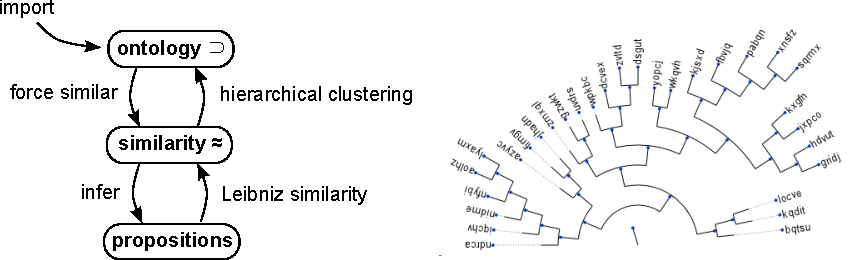
\includegraphics[scale=0.8]{ontology-relations-relations.pdf}
\caption{Left: relations between ontological data.  Right: a random example of dendrogram.}
\label{fig:ontology-relations-relations}
\end{figure}

\section*{Appendix: XXXX}

\section*{Acknowledgments}

I am heavily indebted to Pei Wang \cite{Wang2006} \cite{Wang2013} and Ben Goertzel \cite{Goertzel2011} for their seminal contributions to AGI.  To Abram Demski and Russell Wallace -- we have spent years exploring many ideas in logic.  Also thanks to Matt Mahoney, Jeff Thompson for discussions of the draft.  William Taysom, Seh, and Joseph Cheung helped implement the code.

\end{comment}

\bibliographystyle{plain} % or number or aaai ...
\bibliography{AGI-book}

\onecolumn

% Bigger figures

\end{document}
